%% bare_conf.tex
%% V1.3
%% 2007/01/11
%% by Michael Shell
%% See:
%% http://www.michaelshell.org/
%% for current contact information.
%%
%% This is a skeleton file demonstrating the use of IEEEtran.cls
%% (requires IEEEtran.cls version 1.7 or later) with an IEEE conference paper.
%%
%% Support sites:
%% http://www.michaelshell.org/tex/ieeetran/
%% http://www.ctan.org/tex-archive/macros/latex/contrib/IEEEtran/
%% and
%% http://www.ieee.org/
%
%%*************************************************************************
%% Legal Notice:
%% This code is offered as-is without any warranty either expressed or
%% implied; without even the implied warranty of MERCHANTABILITY or
%% FITNESS FOR A PARTICULAR PURPOSE!
%% User assumes all risk.
%% In no event shall IEEE or any contributor to this code be liable for
%% any damages or losses, including, but not limited to, incidental,
%% consequential, or any other damages, resulting from the use or misuse
%% of any information contained here.
%%
%% All comments are the opinions of their respective authors and are not
%% necessarily endorsed by the IEEE.
%%
%% This work is distributed under the LaTeX Project Public License (LPPL)
%% ( http://www.latex-project.org/ ) version 1.3, and may be freely used,
%% distributed and modified. A copy of the LPPL, version 1.3, is included
%% in the base LaTeX documentation of all distributions of LaTeX released
%% 2003/12/01 or later.
%% Retain all contribution notices and credits.
%% ** Modified files should be clearly indicated as such, including  **
%% ** renaming them and changing author support contact information. **
%%
%% File list of work: IEEEtran.cls, IEEEtran_HOWTO.pdf, bare_adv.tex,
%%                    bare_conf.tex, bare_jrnl.tex, bare_jrnl_compsoc.tex
%%*************************************************************************

% *** Authors should verify (and, if needed, correct) their LaTeX system  ***
% *** with the testflow diagnostic prior to trusting their LaTeX platform ***
% *** with production work. IEEE's font choices can trigger bugs that do  ***
% *** not appear when using other class files.                            ***
% The testflow support page is at:
% http://www.michaelshell.org/tex/testflow/



% Note that the a4paper option is mainly intended so that authors in
% countries using A4 can easily print to A4 and see how their papers will
% look in print - the typesetting of the document will not typically be
% affected with changes in paper size (but the bottom and side margins will).
% Use the testflow package mentioned above to verify correct handling of
% both paper sizes by the user's LaTeX system.
%
% Also note that the "draftcls" or "draftclsnofoot", not "draft", option
% should be used if it is desired that the figures are to be displayed in
% draft mode.
%
\documentclass[10pt, conference, compsocconf]{IEEEtran}
% Add the compsocconf option for Computer Society conferences.
%
% If IEEEtran.cls has not been installed into the LaTeX system files,
% manually specify the path to it like:
% \documentclass[conference]{../sty/IEEEtran}





% Some very useful LaTeX packages include:
% (uncomment the ones you want to load)


% *** MISC UTILITY PACKAGES ***
%
%\usepackage{ifpdf}
% Heiko Oberdiek's ifpdf.sty is very useful if you need conditional
% compilation based on whether the output is pdf or dvi.
% usage:
% \ifpdf
%   % pdf code
% \else
%   % dvi code
% \fi
% The latest version of ifpdf.sty can be obtained from:
% http://www.ctan.org/tex-archive/macros/latex/contrib/oberdiek/
% Also, note that IEEEtran.cls V1.7 and later provides a builtin
% \ifCLASSINFOpdf conditional that works the same way.
% When switching from latex to pdflatex and vice-versa, the compiler may
% have to be run twice to clear warning/error messages.






% *** CITATION PACKAGES ***
%
%\usepackage{cite}
% cite.sty was written by Donald Arseneau
% V1.6 and later of IEEEtran pre-defines the format of the cite.sty package
% \cite{} output to follow that of IEEE. Loading the cite package will
% result in citation numbers being automatically sorted and properly
% "compressed/ranged". e.g., [1], [9], [2], [7], [5], [6] without using
% cite.sty will become [1], [2], [5]--[7], [9] using cite.sty. cite.sty's
% \cite will automatically add leading space, if needed. Use cite.sty's
% noadjust option (cite.sty V3.8 and later) if you want to turn this off.
% cite.sty is already installed on most LaTeX systems. Be sure and use
% version 4.0 (2003-05-27) and later if using hyperref.sty. cite.sty does
% not currently provide for hyperlinked citations.
% The latest version can be obtained at:
% http://www.ctan.org/tex-archive/macros/latex/contrib/cite/
% The documentation is contained in the cite.sty file itself.






% *** GRAPHICS RELATED PACKAGES ***
%


\ifCLASSINFOpdf
  % \usepackage[pdftex]{graphicx}
  % declare the path(s) where your graphic files are
  % \graphicspath{{../pdf/}{../jpeg/}}
  % and their extensions so you won't have to specify these with
  % every instance of \includegraphics
  % \DeclareGraphicsExtensions{.pdf,.jpeg,.png}
\else
  % or other class option (dvipsone, dvipdf, if not using dvips). graphicx
  % will default to the driver specified in the system graphics.cfg if no
  % driver is specified.
  % \usepackage[dvips]{graphicx}
  % declare the path(s) where your graphic files are
  % \graphicspath{{../eps/}}
  % and their extensions so you won't have to specify these with
  % every instance of \includegraphics
  % \DeclareGraphicsExtensions{.eps}
\fi
% graphicx was written by David Carlisle and Sebastian Rahtz. It is
% required if you want graphics, photos, etc. graphicx.sty is already
% installed on most LaTeX systems. The latest version and documentation can
% be obtained at:
% http://www.ctan.org/tex-archive/macros/latex/required/graphics/
% Another good source of documentation is "Using Imported Graphics in
% LaTeX2e" by Keith Reckdahl which can be found as epslatex.ps or
% epslatex.pdf at: http://www.ctan.org/tex-archive/info/
%
% latex, and pdflatex in dvi mode, support graphics in encapsulated
% postscript (.eps) format. pdflatex in pdf mode supports graphics
% in .pdf, .jpeg, .png and .mps (metapost) formats. Users should ensure
% that all non-photo figures use a vector format (.eps, .pdf, .mps) and
% not a bitmapped formats (.jpeg, .png). IEEE frowns on bitmapped formats
% which can result in "jaggedy"/blurry rendering of lines and letters as
% well as large increases in file sizes.
%
% You can find documentation about the pdfTeX application at:
% http://www.tug.org/applications/pdftex





% *** MATH PACKAGES ***
%
%\usepackage[cmex10]{amsmath}
% A popular package from the American Mathematical Society that provides
% many useful and powerful commands for dealing with mathematics. If using
% it, be sure to load this package with the cmex10 option to ensure that
% only type 1 fonts will utilized at all point sizes. Without this option,
% it is possible that some math symbols, particularly those within
% footnotes, will be rendered in bitmap form which will result in a
% document that can not be IEEE Xplore compliant!
%
% Also, note that the amsmath package sets \interdisplaylinepenalty to 10000
% thus preventing page breaks from occurring within multiline equations. Use:
%\interdisplaylinepenalty=2500
% after loading amsmath to restore such page breaks as IEEEtran.cls normally
% does. amsmath.sty is already installed on most LaTeX systems. The latest
% version and documentation can be obtained at:
% http://www.ctan.org/tex-archive/macros/latex/required/amslatex/math/





% *** SPECIALIZED LIST PACKAGES ***
%
%\usepackage{algorithmic}
% algorithmic.sty was written by Peter Williams and Rogerio Brito.
% This package provides an algorithmic environment fo describing algorithms.
% You can use the algorithmic environment in-text or within a figure
% environment to provide for a floating algorithm. Do NOT use the algorithm
% floating environment provided by algorithm.sty (by the same authors) or
% algorithm2e.sty (by Christophe Fiorio) as IEEE does not use dedicated
% algorithm float types and packages that provide these will not provide
% correct IEEE style captions. The latest version and documentation of
% algorithmic.sty can be obtained at:
% http://www.ctan.org/tex-archive/macros/latex/contrib/algorithms/
% There is also a support site at:
% http://algorithms.berlios.de/index.html
% Also of interest may be the (relatively newer and more customizable)
% algorithmicx.sty package by Szasz Janos:
% http://www.ctan.org/tex-archive/macros/latex/contrib/algorithmicx/




% *** ALIGNMENT PACKAGES ***
%
%\usepackage{array}
% Frank Mittelbach's and David Carlisle's array.sty patches and improves
% the standard LaTeX2e array and tabular environments to provide better
% appearance and additional user controls. As the default LaTeX2e table
% generation code is lacking to the point of almost being broken with
% respect to the quality of the end results, all users are strongly
% advised to use an enhanced (at the very least that provided by array.sty)
% set of table tools. array.sty is already installed on most systems. The
% latest version and documentation can be obtained at:
% http://www.ctan.org/tex-archive/macros/latex/required/tools/


%\usepackage{mdwmath}
%\usepackage{mdwtab}
% Also highly recommended is Mark Wooding's extremely powerful MDW tools,
% especially mdwmath.sty and mdwtab.sty which are used to format equations
% and tables, respectively. The MDWtools set is already installed on most
% LaTeX systems. The lastest version and documentation is available at:
% http://www.ctan.org/tex-archive/macros/latex/contrib/mdwtools/


% IEEEtran contains the IEEEeqnarray family of commands that can be used to
% generate multiline equations as well as matrices, tables, etc., of high
% quality.


%\usepackage{eqparbox}
% Also of notable interest is Scott Pakin's eqparbox package for creating
% (automatically sized) equal width boxes - aka "natural width parboxes".
% Available at:
% http://www.ctan.org/tex-archive/macros/latex/contrib/eqparbox/





% *** SUBFIGURE PACKAGES ***
\usepackage[footnotesize]{subfigure}
%\usepackage[tight,footnotesize]{subfigure}
% subfigure.sty was written by Steven Douglas Cochran. This package makes it
% easy to put subfigures in your figures. e.g., "Figure 1a and 1b". For IEEE
% work, it is a good idea to load it with the tight package option to reduce
% the amount of white space around the subfigures. subfigure.sty is already
% installed on most LaTeX systems. The latest version and documentation can
% be obtained at:
% http://www.ctan.org/tex-archive/obsolete/macros/latex/contrib/subfigure/
% subfigure.sty has been superceeded by subfig.sty.


\usepackage{epsfig}
\usepackage{graphics}
\usepackage{epstopdf}


%\usepackage[caption=false]{caption}
%\usepackage[font=footnotesize]{subfig}
% subfig.sty, also written by Steven Douglas Cochran, is the modern
% replacement for subfigure.sty. However, subfig.sty requires and
% automatically loads Axel Sommerfeldt's caption.sty which will override
% IEEEtran.cls handling of captions and this will result in nonIEEE style
% figure/table captions. To prevent this problem, be sure and preload
% caption.sty with its "caption=false" package option. This is will preserve
% IEEEtran.cls handing of captions. Version 1.3 (2005/06/28) and later
% (recommended due to many improvements over 1.2) of subfig.sty supports
% the caption=false option directly:
%\usepackage[caption=false,font=footnotesize]{subfig}
%
% The latest version and documentation can be obtained at:
% http://www.ctan.org/tex-archive/macros/latex/contrib/subfig/
% The latest version and documentation of caption.sty can be obtained at:
% http://www.ctan.org/tex-archive/macros/latex/contrib/caption/




% *** FLOAT PACKAGES ***
%
%\usepackage{fixltx2e}
% fixltx2e, the successor to the earlier fix2col.sty, was written by
% Frank Mittelbach and David Carlisle. This package corrects a few problems
% in the LaTeX2e kernel, the most notable of which is that in current
% LaTeX2e releases, the ordering of single and double column floats is not
% guaranteed to be preserved. Thus, an unpatched LaTeX2e can allow a
% single column figure to be placed prior to an earlier double column
% figure. The latest version and documentation can be found at:
% http://www.ctan.org/tex-archive/macros/latex/base/



%\usepackage{stfloats}
% stfloats.sty was written by Sigitas Tolusis. This package gives LaTeX2e
% the ability to do double column floats at the bottom of the page as well
% as the top. (e.g., "\begin{figure*}[!b]" is not normally possible in
% LaTeX2e). It also provides a command:
%\fnbelowfloat
% to enable the placement of footnotes below bottom floats (the standard
% LaTeX2e kernel puts them above bottom floats). This is an invasive package
% which rewrites many portions of the LaTeX2e float routines. It may not work
% with other packages that modify the LaTeX2e float routines. The latest
% version and documentation can be obtained at:
% http://www.ctan.org/tex-archive/macros/latex/contrib/sttools/
% Documentation is contained in the stfloats.sty comments as well as in the
% presfull.pdf file. Do not use the stfloats baselinefloat ability as IEEE
% does not allow \baselineskip to stretch. Authors submitting work to the
% IEEE should note that IEEE rarely uses double column equations and
% that authors should try to avoid such use. Do not be tempted to use the
% cuted.sty or midfloat.sty packages (also by Sigitas Tolusis) as IEEE does
% not format its papers in such ways.





% *** PDF, URL AND HYPERLINK PACKAGES ***
%
%\usepackage{url}
% url.sty was written by Donald Arseneau. It provides better support for
% handling and breaking URLs. url.sty is already installed on most LaTeX
% systems. The latest version can be obtained at:
% http://www.ctan.org/tex-archive/macros/latex/contrib/misc/
% Read the url.sty source comments for usage information. Basically,
% \url{my_url_here}.



% *** Do not adjust lengths that control margins, column widths, etc. ***
% *** Do not use packages that alter fonts (such as pslatex).         ***
% There should be no need to do such things with IEEEtran.cls V1.6 and later.
% (Unless specifically asked to do so by the journal or conference you plan
% to submit to, of course. )


% correct bad hyphenation here
%\hyphenation{op-tical net-works semi-conduc-tor}

%\newcommand{\SeTAB}{{\sc SeARuM}}
%\newcommand{\SeTA}{a cloud-based {\sc Se}rvice for network {\sc T}raffic {\sc A}nalysis}
%\newcommand{\SeTA}{a cloud-based {\sc Se}rvice for {\sc A}ssociation {\sc Ru}le {\sc M}ining}
\newcommand{\SeTAB}{{\sc MGI-Cloud}}
\newcommand{\SeTA}{{\sc M}isleading {\sc G}eneralized {\sc I}temset miner in the {\sc Cloud}}
\newcommand{\MGI}{{\sc M}isleading {\sc G}eneralized {\sc I}temset}
\newcommand{\Alg}{{\sc M}isleading {\sc G}eneralized {\sc I}temset {\sc M}iner}

\begin{document}
%
% paper title
% can use linebreaks \\ within to get better formatting as desired
\title{Misleading generalized itemset mining in the cloud}


% author names and affiliations
% use a multiple column layout for up to two different
% affiliations
\IEEEoverridecommandlockouts
\author{\IEEEauthorblockN{Elena Baralis, Luca Cagliero, Tania Cerquitelli, Silvia Chiusano, Paolo Garza, Luigi Grimaudo, Fabio Pulvirenti}
\IEEEauthorblockA{Dipartimento di Automatica e Informatica\\
Politecnico di Torino\\
Torino, Italy\\
Email: \{name.surname\}@polito.it}


\thanks{The research leading to these results has received funding from the European Union 
under the FP7 Grant Agreement n. 285248 (Integrated Project ”FI-WARE”) and 
the FP7 Grant Agreement n. 619633 (Integrated Project ”ONTIC”)} 
}

% conference papers do not typically use \thanks and this command
% is locked out in conference mode. If really needed, such as for
% the acknowledgment of grants, issue a \IEEEoverridecommandlockouts
% after \documentclass

% for over three affiliations, or if they all won't fit within the width
% of the page, use this alternative format:
%
%\author{\IEEEauthorblockN{Michael Shell\IEEEauthorrefmark{1},
%Homer Simpson\IEEEauthorrefmark{2},
%James Kirk\IEEEauthorrefmark{3},
%Montgomery Scott\IEEEauthorrefmark{3} and
%Eldon Tyrell\IEEEauthorrefmark{4}}
%\IEEEauthorblockA{\IEEEauthorrefmark{1}School of Electrical and Computer Engineering\\
%Georgia Institute of Technology,
%Atlanta, Georgia 30332--0250\\ Email: see http://www.michaelshell.org/contact.html}
%\IEEEauthorblockA{\IEEEauthorrefmark{2}Twentieth Century Fox, Springfield, USA\\
%Email: homer@thesimpsons.com}
%\IEEEauthorblockA{\IEEEauthorrefmark{3}Starfleet Academy, San Francisco, California 96678-2391\\
%Telephone: (800) 555--1212, Fax: (888) 555--1212}
%\IEEEauthorblockA{\IEEEauthorrefmark{4}Tyrell Inc., 123 Replicant Street, Los Angeles, California 90210--4321}}

% use for special paper notices
%\IEEEspecialpapernotice{(Invited Paper)}


% make the title area
\maketitle


\begin{abstract}
In the era of smart cities huge data volumes are continuously generated and collected, thus prompting the need for efficient 
and distributed data mining approaches. 
Generalized itemset mining is an established data mining technique, which entails the discovery of multiple-level patterns 
hidden in the analyzed data by exploiting analyst-provided taxonomies.
Among the generalized itemsets, the most peculiar high-level patterns are those with many contrasting correlations among items at different abstraction levels. 
They represent misleading situations that are worth analyzing separately by experts during manual inspection.

This paper proposes a novel cloud-based service, named \SeTAB,
to efficiently mine misleading multiple-level patterns, i.e., the Misleading Generalized Itemsets, on a distributed computing environment.
\SeTAB\ consists of a set of distributed MapReduce jobs running in the cloud.
As a case study, the system has been contextualized in a real-life scenario, i.e., the analysis of traffic law infractions committed in a smart city environment.
The experiments, performed on real datasets, demonstrate the efficiency and effectiveness of \SeTAB. 



\end{abstract}

\begin{IEEEkeywords}
Generalized itemset mining; distributed computing model; cloud-based service; smart city.
\end{IEEEkeywords}

\IEEEpeerreviewmaketitle



\section{Introduction}

In the last few years the new Information and Communication Technologies (ICT) have supported cities in becoming smart.
Hence, the capability of smart cities to generate and collect data of public interest (e.g., information about social events, public service usage, traffic law infractions) has increased at an unprecedented rate, 
to such an extent that data rapidly scales towards ``Big Data''. 

Big Data analyses are challenging tasks because the computational cost of data mining processes is often very high and, in some cases, prohibitive
on a non-distributed system.  Hence, relevant research efforts have been devoted to large-scale data mining based on the MapReduce paradigm~\cite{Dean2008}.
Data mining encompasses a large variety of techniques, such as cluster analysis, frequent pattern extraction, and classification~\cite{KumarBook}. 
For example, some remarkable attempts to address itemset and association rule mining from Big Data have recently been made (e.g.,~\cite{pfpgrowth,bigfim,ISPA13,PMINE13}). 
This paper focuses on an established pattern mining technique called generalized itemset extraction~\cite{Srikant1995}. 
This technique has already been applied to data coming from different application domains (e.g., market basket analysis~\cite{Srikant1995}, network traffic data analysis~\cite{IS2010}, genetic data mining~\cite{BaralisCCCG13}). 
Generalized itemset mining entails discovering correlations among data at different abstraction levels. By exploiting a taxonomy (i.e., a set of is-a hierarchies) built over the analyzed data, 
frequent generalized itemsets, which represent recurrent co-occurrences among data items at different granularity levels, are extracted. 
These patterns are worth considering by domain experts to transform huge amounts of raw data into useful and actionable knowledge. 
However, a subset of peculiar high-level patterns should be analyzed separately during manual result inspection.  
More specifically, each generalized itemset has a correlation type which indicates the strength of the correlation between the corresponding items. 
Misleading Generalized Itemsets (MGIs)~\cite{MGI} are generalized itemsets
whose correlations type is in contrast to those of most of their low-level descendant itemsets.
These high-level patterns are worth considering for in-depth analysis because they are likely to represent misleading and thus potentially interesting situations. 
In~\cite{MGI} MGI extraction is performed in main memory on top of frequent level-sharing itemsets. 
Unfortunately, when coping with Big Datasets, a large number of itemsets is often generated at step (i) thus MGI extraction becomes a challenging task. 
However, to the best of our knowledge, no attempt to mine MGIs on a distributed architecture has been made yet. 

This paper presents a cloud-based service, named \SeTAB\ (\SeTA ), to efficiently mine MGIs on a distributed computing model. 
To efficiently cope with Big Data collections, the system implementation is distributed and most operations are mapped to the MapReduce programming paradigm~\cite{Dean2008}. 
As a reference case study, the proposed approach has been applied to a real application context: the analysis of the traffic law infractions committed by 
the citizens of Turin, an important business and cultural centre in northern Italy. 
Real infraction data is provided as open data by the Turin administration.
The goal of the analysis is to improve the efficiency of public services, 
the transparency of public administrations, and the awareness of the degree of civilization of urban people.
The experimental results show the effectiveness and efficiency of the \SeTAB\ architecture as well as they demonstrate its applicability to the analyzed use-case. 

The paper is organized as follows. Section~\ref{relwork} overviews most relevant previous works. 
Section~\ref{probstat} states the problem addressed in this
paper. Section~\ref{setarch} presents the \SeTAB\ architecture while a preliminary experimental evaluation of our approach is reported in Section~\ref{exp}. Finally,
Section~\ref{conclusion} draws conclusions and discusses future research directions.

%*********************************************************
\section{Related work}
\label{relwork}
%*********************************************************

In the last years, a relevant research effort has been devoted to large-scale itemset mining based on the MapReduce paradigm~\cite{Dean2008}. 
The goal is to propose itemset extraction algorithms that distribute data and computation across a distributed architecture to scale the mining process towards Big Data~\cite{pfpgrowth,bigfim,ISPA13}.
A parallel version of an established itemset mining algorithm, i.e., FP-Growth, has first been proposed in~\cite{pfpgrowth}. 
The algorithm, named PFP, consists of two separate MapReduce jobs 
and it achieves an almost linear speedup.
It converts transactions of the original database into some new databases of group-dependent transactions so that local FP-trees built
from different group-dependent transactions can be separately processed during the recursive conditional FP-tree constructing process. 
For each group PFP extracts top-k frequent itemsets (i.e., a subset of frequent itemsets).
More recently, two new methods, namely Dist-Eclat and BigFIM, for mining all frequent itemsets from large datasets 
have been presented in~\cite{bigfim}. 
Specifically, Dist-Eclat focuses on improving algorithm speed, while BigFIM is optimized to run on huge datasets.
In parallel, a cloud-based service for association rule mining from network traffic data has been presented in~\cite{ISPA13}.
Unlike~\cite{pfpgrowth,bigfim,ISPA13}, this paper investigates the applicability of a generalized pattern mining technique on the MapReduce platform. 

The frequent generalized frequent itemset and association rule mining problems~\cite{Srikant1995} have largely been studied by the data mining community.
The firstly proposed approach~\cite{Srikant1995} generates itemsets by considering for each item all its ancestors in the taxonomy. 
To avoid generating all the possible itemsets, the authors in~\cite{Sriphaew2002,BaralisCCG12} proposed to push (analyst-provided) constraints into the mining process.
In parallel, many algorithm optimizations and variations have been proposed~\cite{Han1999,KunkleZC08,ChangeTKDE}. 
For example, the approach presented in~\cite{Han1999} proposes an optimization strategy based on a top-down hierarchy traversal, while 
in~\cite{KunkleZC08} the authors propose to mine closed and maximal generalized itemsets. 
More recently, a new type of generalized pattern, called Misleading Generalized Itemset (MGI), has been proposed~\cite{MGI}. 
MGIs are high-level (generalized) itemsets for which a relevant subset of frequent descendants have a correlation type in contrast to their common ancestor. 
MGIs are worth considering separately from traditional itemsets if their low-level contrasting correlations cover almost the same portion of data as the high-level itemset, 
because the information provided by traditional high-level patterns becomes misleading. 
Unlike~\cite{MGI}, this paper investigates how to perform MGI mining on the MapReduce platform. 
Furthermore, it presents a cloud-based service for discovering MGIs from Big Data acquired in smart city environments.


%**********************************************************
\section{Preliminary concepts and problem statement}
\label{probstat}
%**********************************************************

A relational dataset $\cal{D}$ consists of a set of records, where each record is a set of items~\cite{KumarBook}. Each item is a pair ($attribute$,~$value$).
A taxonomy $\Gamma$ built over the source dataset $\cal{D}$  aggregates the data items into higher-level concepts (i.e., the generalized items). 
Table~\ref{tab:example2} and Table~\ref{fig:tax} report two representative examples of relational dataset and taxonomy, respectively, which hereafter will be used as running examples. 

\begin{table*}%
\parbox{0.42\textwidth}{
\caption{Example dataset $\cal{D}$ after discretization.}
\begin{scriptsize}
\begin{center}
\begin{tabular}{|c||c|c|}
\hline {\bf Rid} & {\bf Infraction name} & {\bf time stamp} \\
\hline
\hline 1 & One-way infraction & [8 a.m.,9 a.m.] \\
\hline 2 & One-way infraction & [8 a.m.,9 a.m.] \\
\hline 3 & Speeding & [8 a.m.,9 a.m.] \\
\hline 4 & Driving without license & [9 a.m.,10 a.m.] \\
\hline 5 & Driving without license & [9 a.m.,10 a.m.] \\
\hline 6 & Unfastened seat belt & [4 p.m.,5 p.m.] \\
\hline 7 & One-way infraction & [8 a.m.,9 a.m.] \\
\hline
\end{tabular}
\end{center}
\end{scriptsize}
\label{tab:example2}
\vspace{1cm}
}
\qquad
\begin{minipage}[c]{0.37\textwidth}%
\centering
\caption{Example taxonomy built over items in $\cal{D}$}
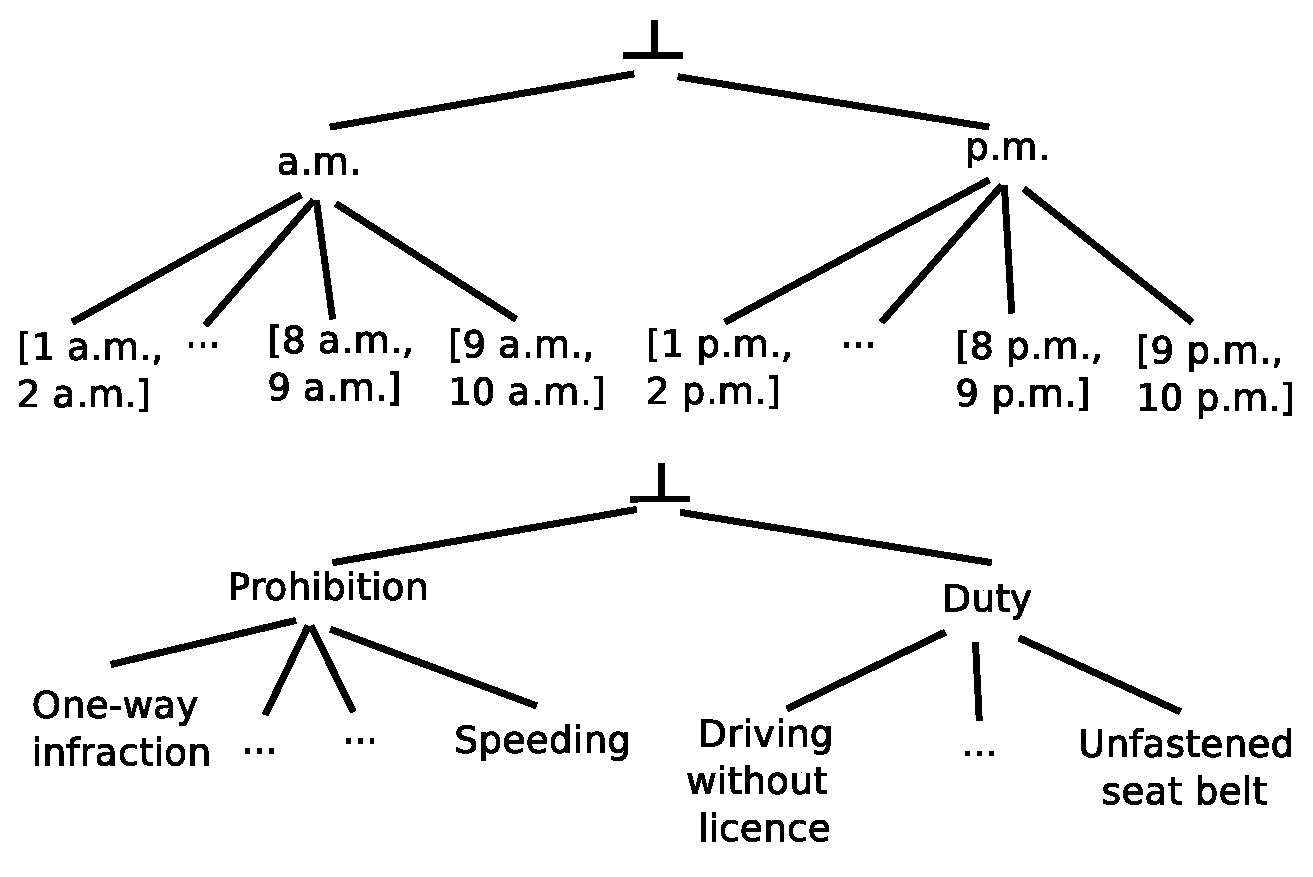
\includegraphics[width=\textwidth]{gerarchia/GerarchiaISPATre.eps}
\label{fig:tax}
\end{minipage}
\end{table*}


\begin{table*}[th!]
\scriptsize
\caption{\MGI{}s mined from $\cal{D}$. min\_sup = 10\%, max\_neg\_cor= 0.70, min\_pos\_cor= 0.80, and max\_NOD = 80\%.} \label{tab:exampleMGI}
\centering
\hspace{-1.5cm}
\begin{tabular}{|c|c|c|}
\hline 
 {\bf Frequent}       		& {\bf Frequent}                   & {\bf Not }    \\
 {\bf itemset (level$\geq$2)}    		& {\bf descendants}                 & {\bf overlapping} \\
 {\bf [correlation type (Kulc value)]}   	& {\bf [correlation type (Kulc value)]} &  {\bf degree (\%)}         \\
\hline
$\{$ (Time, a.m.), (Infraction name, Prohibition)$\}$    &   $\{$(Time, [8 a.m.,9 a.m.]), (Infraction name, One-way infraction)$\}$ & 75   \\
     \textit{[positive (5/6=0.83)]}       &    \textit{[positive (7/8=0.88)]}         &  \\
                                 &  $\{$(Time, [8 a.m.,9 a.m.]), (Infraction name, Speeding)$\}$    &  \\
                                 &    \textit{[[negative (5/8=0.63)]}              &  \\
\hline
 $\{$(Time, a.m.), (Infraction name, Duty)$\}$  &  $\{$(Time, [9 a.m., 10 a.m.]), (Infraction name, Driving without license)$\}$  & 0  \\
           \textit{[negative (1/2=0.50)]}                  & \textit{[positive (1)]} &  \\        
\hline
 $\{$(Time, p.m.), (Infraction name, Duty)$\}$  &  $\{$(Time, [4 p.m.,5 p.m.]), (Infraction name, Unfastened seat belt)$\}$  & 0   \\
           \textit{[negative (2/3=0.66)]}                  &  \textit{[positive (1)]} &  \\
\hline
\end{tabular}
\end{table*}

A $k$-itemset is a set of $k$ (generalized) items. 
For example, \{(\textit{Time},\textit{a.m.}), (\textit{Infraction name},\textit{One-way infraction})\} is a $2$-itemset, 
which indicates that the two items co-occur (possibly at different abstraction levels) in the source data.  
Items/itemsets are characterized by many notable properties~\cite{Srikant1995}, such as support, coverage, descent and level of abstraction according to an input taxonomy $\Gamma$. 
For their definitions please refer to~\cite{Srikant1995,Han1999,MGI}. 
Similar to~\cite{Han1999,Flipping}, we target the correlations among items at same abstraction level, i.e. the itemsets that exclusively contain items with the same level. Such patterns are denoted by \textit{level-sharing itemsets}~\cite{Han1999}. 

The itemset correlation measures the strength of the correlation between its items. Similar to~\cite{Flipping}, in this paper
we evaluate the correlation of a $k$-itemset $I$ by means of the Kulczynsky (Kulc) correlation measure~\cite{Wu2010Interestingness}
Kulc values range from 0 to 1. By properly setting maximum negative and minimum positive
Kulc thresholds, hereafter denoted by \textit{max\_neg\_cor} and \textit{min\_pos\_cor}, the itemsets may be classified as negatively correlated, uncorrelated, or positively correlated itemsets according to their correlation value.  

Let $\mathcal{LSI}$ be the set of all frequent level-sharing itemsets in $\mathcal{D}$ according to a minimum support threshold min\_sup. 
Given a frequent level-sharing itemset $X \in \mathcal{LGI}$ of level $l\geq2$, let 
Desc$^*$[$X$,$\Gamma$] be the subset of corresponding level-($l-1$) $X$'s descendants for which the correlation type is in contrast to those of $X$. 
A \MGI\ (MGI) is a pattern in the form $X \triangleright \mathcal{E}$, where $X \in \mathcal{LSGI}$ and $\mathcal{E}$=Desc$^*$[$X$,$\Gamma$]~\cite{MGI}. 

For example, by enforcing min\_sup=10\%, max\_neg\_cor=0.70, 
and min\_pos\_cor=0.80, MGI
\{(Time,a.m.), (Infraction name,Prohibition)\}~$\triangleright$~\{(Time, [8 a.m.,9 a.m.]), (Infraction name,Speeding)\} is 
mined from the dataset in Table~\ref{tab:example2}, 
because \{(Time,a.m.), (Infraction name,Prohibition)\} has a positive correlation (0.83), 
whereas its descendant itemset \{(Time,[8 a.m., 9 a.m.]), (Infraction name,Speeding)\} is negatively correlated (0.63).

To measure the degree of interest of a MGI $X \triangleright \mathcal{E}$ with respect to its corresponding traditional itemset version ($X$), 
the Not Overlapping Degree (NOD) measure has been defined in~\cite{MGI}. 
The NOD of an MGI $X \triangleright \mathcal{E}$ is defined as 
$\frac{\mbox{sup}(X,\cal{D})-\mbox{cov}(\mathcal{E},\cal{D})}{\mbox{sup}(X,\cal{D})}$.
It expresses the relative difference between the support of the ancestor itemset $X$ and the coverage of its low-level contrasting correlations in $\mathcal{E}$.
The NOD values range from 0 to 1. The lower NOD value we achieve, the more significant the degree of overlapping between 
the contrasting low-level correlations in $\mathcal{E}$ and their common ancestor $X$ becomes. 

The mining task addressed by this paper entails discovering from $\cal{D}$ all the MGIs for which
the NOD value is less than or equal to a maximum threshold max\_NOD. The subset of \MGI s mined from Table~\ref{tab:example2} by setting the maximum NOD threshold to 80\% is reported in Table~\ref{tab:exampleMGI}.




%**********************************************************
\section{The \SeTAB\ architecture}
\label{setarch}
%**********************************************************

The \SeTAB\ architecture provides a cloud-based service for discovering hidden and actionable patterns among potentially Big datasets.
We focus our analysis on a specific case study, i.e., the analysis of the traffic law infractions committed in a urban environment. 
To efficiently cope with Big Data, the system implementation is distributed and most operations are mapped to the MapReduce programming paradigm~\cite{Dean2008}.
The architecture has been designed as a chain of distributed jobs running on an Hadoop cluster, as described below. 


%**********************************************
\subsection{Data retrieval and preparation}
\label{acquisitionprep}
%**********************************************

Data about traffic law infractions was collected by traffic engineers. 
Reports about daily infractions are collected in local data repositories, which are then integrated into open Big Datasets. 
A traffic law infraction dataset $\mathcal{D}$ consists of a set of records $r$, each one representing a different infraction. 
Each record is a set of \textit{items}, where items are pairs (\textit{attribute},\textit{value}). \
\textit{Attribute} can be a specific characteristic of the traffic law infraction (e.g.,  infraction name, law article) 
or a property of the context in which the infraction was committed (location, date, time), 
while \textit{value} is the value assumed by the corresponding attribute. 
Hereafter, for the sake of simplicity, we focus our analysis on the following attribute subset: \textit{Infraction name}, \textit{Vehicle type}, \textit{Location}, \textit{Date}, and \textit{Time}. 
We discretized time stamps (e.g., 8.10 a.m.) into 1-hour time slots (e.g., from 8 a.m. to 9 a.m.) using ad-hoc mapping functions. 
The dataset reported in Table~\ref{tab:example2} is already the output of the discretization step.
Attribute selection and data discretization are performed as distributed MapReduce jobs.


%**********************************************
\subsection{Taxonomy generation}
\label{taxmapping}
%**********************************************

To analyze data from a high-level viewpoint, real infraction datasets are equipped with taxonomies.
A taxonomy is a set of is-a hierarchies built over data items in $\mathcal{D}$. 
An example taxonomy built over the dataset in Table~\ref{tab:example2} is depicted in Table~\ref{fig:tax}. 
Items whose value is an high-level aggregation belonging to the taxonomy (e.g., (\textit{Infraction name},\textit{Duty})) are called \textit{generalized items}. 

Analyst-provided taxonomies could be generated either manually or semi-automatically by domain experts. 
To perform our analyzes, we built 3-level hierarchies over the contextual attributes (Location, Time, Date). Specifically, geographical addresses 
are aggregated into the zip code, which in turn are aggregated into the corresponding district; 1-hour time slots are generalized as the corresponding 4- and 12-hour time slots, 
while dates are generalized as the corresponding month and year.
Furthermore, vehicles are generalized as the corresponding category (e.g., \textit{Car}, \textit{Dumper track}, \textit{Pickup track}), and
infraction names are aggregated into the corresponding high-level class given by the public administration of Turin.
In this work we consider as input balanced taxonomies (i.e., taxonomies whose hierarchies have all the same height). 
If experts do not provide balanced taxonomies, a re-balancing procedure similar to those adopted in~\cite{Flipping} is applied prior to level-sharing itemset mining.  


%**********************************************
\subsection{Level-sharing itemset mining}
\label{levelsharing}
%**********************************************


Given a preprocessed infraction dataset and a minimum support threshold min\_sup, this job accomplishes the first MGI mining step, i.e., the extraction of all frequent level-sharing itemsets~\cite{Han1999}.  
This job performs the following tasks. 

\noindent \textbf{Dataset extension}. This task entails producing a new dataset version which integrates taxonomy information. 
To enable frequent level-sharing itemset mining from data containing items at different abstraction levels, it generates multiple copies of each record, one for each taxonomy level. 
While the original record contains only taxonomy leaves (i.e., the dataset items), each copy contains the corresponding combination of item generalizations at a different abstraction level.To avoid unnecessary I/O operations, the extended dataset version is not materialized on disk, but it is directly 
generated in the map function of the itemset extraction task and then immediately stored into a compact FP-tree structure~\cite{KumarBook}.

\noindent \textbf{Itemset extraction}. To efficiently mine frequent level-sharing itemsets~\cite{Han1999} from the extended dataset version, 
this task exploits a variation of the Hadoop-based itemset mining algorithm proposed in~\cite{ISPA13}. 


%**********************************************************
\subsection{MGI extraction}
\label{rulext}
%**********************************************************

This job performs MGI mining on top of the frequent level-sharing itemsets. 
Specifically, it accomplishes the task stated in Section~\ref{probstat}. 
This step consists of a MapReduce job, as described in the following.
The contribution of this job is new because, to the best of our knowledge, no cloud-based service currently supports MGI mining from Big Data.

To extract MGIs we combine each frequent level-sharing itemset $I$ with  
its corresponding set of descendant itemsets $\mbox{Desc}[I,\Gamma]$. 
More specifically, In the map function for each level-sharing itemset $I$, the following two pairs ($key$, $value$) are emitted:
(i) a pair ($key$, $value$), where $key$ is the direct ancestor of itemset $I$ and $value$ the itemset $I$ with its main properties (i.e., support and Kulc values) and
(ii) a pair ($key$, $value$), where $key$ is the itemset $I$ is the $value$: itemset $I$ with its main properties (i.e., support and Kulc values).
Two pairs are emitted because each itemset can be a descendant of an itemset and 
a parent of another one at the same time. The first pair allows us to associate $I$ with the ancestor key, whereas
the second pair is used to associate $I$ to itself if MGIs in the form $I \triangleright \mathcal{E}$ are extracted. 
The generated pairs allow us to map each itemset and its corresponding descendants to the same key. 
Hence, in the reduce function, each key is associated with a specific itemset $I$ and the corresponding set of values 
contains both the (ancestor) itemset $I$ and its respective descendants. By iterating on the set of values associated with key $I$, 
we generate candidate MGIs $I \triangleright \mathcal{E}$, where $\mathcal{E}$ is the set of $I$'s descendants in contrast to $I$ in terms of correlation type,
and we compute the corresponding NOD values. Finally, only the MGIs satisfying the max\_NOD threshold are stored into the HDFS file system.


%**********************************************************
\section{Experiments}
\label{exp}
%**********************************************************
We performed experiments on two real datasets acquired in different domains:

\noindent \textbf{AperTo dataset.}  This open dataset, available at http://aperto.comune.torino.it, collects information about approximately 2 millions of traffic law infractions committed in the city 
of Turin over the 3-year period 2011-2013. The dataset is characterized by five attributes (\textit{Infraction name}, \textit{Vehicle type}, \textit{Location}, \textit{Date}, and \textit{Time}). Its size is approximately 198 MB. 
Hierarchies over the infraction data items were defined according to the guidelines reported in Section~\ref{taxmapping}.

\noindent  \textbf{BigNetData dataset.} This relational network traffic dataset has been obtained by performing different
capture stages on a backbone link of a nation-wide ISP in Italy that offers us three different vantage points.
The dataset has size 192.56 GB and it consists of 413,012,989 records, i.e., one record for each bi-directional TCP flow).
A more detailed dataset description is given in~\cite{ISPA13}.

The MapReduce jobs of the \SeTAB\ workflow (see Section~\ref{setarch}) were
developed in Java using the new Hadoop Java APIs.
The experiments were performed on a cluster of 5 nodes running Cloudera's
Distribution of Apache Hadoop (CDH4.5). Each cluster node is a 2.67~GHz
six-core Intel(R) Xeon(R) X5650 machine with 32~Gbyte of main memory running
Ubuntu 12.04 server with the 3.5.0-23-generic kernel. All the reported
execution times are real times obtained from the Cloudera Manager web control panel.

In the experiments we addressed the following issues: 
(i) the analysis of the characteristics of the mining results achieved with different parameter settings ((Section~\ref{impactparam})), 
(ii) the validation of the usefulness of the results achieved for performing in-depth analysis (Section~\ref{validation}), 
and (iii)~the scalability of the MGI Miner algorithm with the number of nodes (Section~\ref{scalability}). 
We addressed Tasks (i) and (ii) on AperTo, because data fully complies with the context under analysis (i.e., infraction data analysis), whereas
Task (iii) was addressed on BiGNetData, because it is a larger dataset characterized by a fairly complex data distribution.

%**********************************************************
\subsection{Characteristics of the mining results}
\label{impactparam}
%**********************************************************

\begin{figure}[t]
\centering
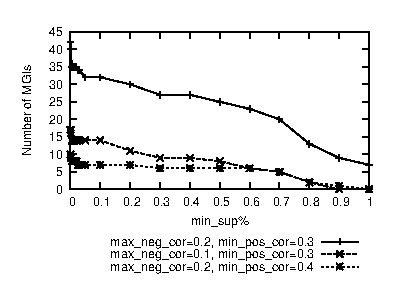
\includegraphics[width=0.32\textwidth]{grafici/EffectMinsup.eps}
\caption{Effect of the minimum support threshold. max\_NOD=60\%.}
\label{fig:minsup}
\end{figure}

\begin{figure}[t]
\centering
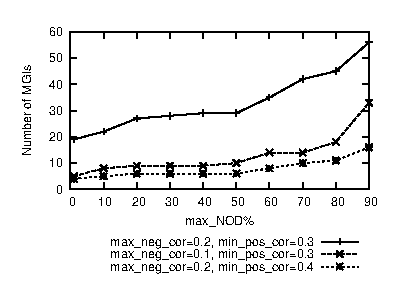
\includegraphics[width=0.32\textwidth]{grafici/EffectMaxNOD.eps}
\caption{Effect of the maximum NOD threshold. minsup=0.02\%.}
\label{fig:maxnod}
\end{figure}

We analyzed the impact of the main input parameters of the MGI Miner algorithm on the number of MGIs mined.
Figure~\ref{fig:minsup} summarizes the number of mined MGIs by varying the minimum support threshold (min\_sup) for different combinations of minimum positive and maximum negative correlation thresholds (max\_neg\_cor and  min\_pos\_cor, respectively), 
while Figure~\ref{fig:maxnod} shows the number of mined MGIs by varying the max\_NOD threshold for the same combinations of correlation threshold values.

The number of mined MGIs non-linearly increases by decreasing the minimum support threshold due to the combinatorial increase in the number of generated frequent itemsets~\cite{Agr94}. 
Since most itemsets have correlation between 0.1 and 0.3, the maximum number of MGIs is extracted if max\_neg\_cor and min\_pos\_cor fall in this value range, 
because the generalization process is most likely to flip the itemset correlation types. As expected, the smaller the gap between max\_neg\_cor and min\_pos\_cor, 
the more MGIs are extracted because correlation type changes occur, on average, more frequently. 
For all the tested configurations, the set of mined MGIs remains still manageable by domain experts for manual inspection even while setting relatively low support thresholds (e.g., 35 MGIs mined with max\_neg\_cor=0.2, min\_pos\_cor=0.3 and min\_sup=0.01\%). 

The number of mined MGIs non-linearly increases while increasing the maximum not overlapping degree threshold max\_NOD, because low-level itemsets are more likely to cover a significant portion of data already covered by the corresponding high-level itemsets. 
However, in all the performed experiments the set of MGIs, which represent anomalies/contrasting situations, remains easily manageable by domain experts for manual exploration. 

%**********************************************************
\subsection{Result validation}
\label{validation}
%**********************************************************

We examined the MGIs extracted from the AperTo dataset to validate their interestingness and usefulness in a real-life context, 
i.e., the analysis of the traffic law infractions committed in a urban environment.

As a first example, let us consider the following MGI extracted by enforcing min\_sup=0.02\%, max\_neg\_cor=0.1, min\_pos\_cor=0.4, and max\_NOD=60\%:
\{(Location,Zip code 10125), (Infraction name,Prohibition)\} $\triangleright$ \{(Location, Sommeiller Avenue), (Infraction name, One-way infraction)\}.
The high-level itemset \{(Location,Zip Code 10125), (Infraction name,Prohibition)\} is negatively correlated, whereas its frequent descendant \{(Location, Sommeiller Avenue), (Infraction name, One-way infraction)\} is positively correlated
and it covers a significant portion of data already covered by the high-level itemset ($\sim$59\%). Hence, to a certain extent, analyzing only 
the traditional high-level itemset instead of the complete MGI could be misleading.
This pattern indicates that in a certain area of Turin, identified by zip code 10125, a category of infractions (prohibitions) is not very likely to occur, 
whereas for a specific avenue within the area wrong way driving prohibition is violated more commonly than expected. Hence, road signs in Sommeiller Avenue could be either not well visible or misplaced. 
The public administration of Turin should deem such information to be worthy for signage maintenance and monitoring.

Let us consider now the following MGI: \{(Location,District 1), (Vehicle type,Private car),(Time, p.m.)\} $\triangleright$ \{(Location, Zip code~10122),(Vehicle type, Private car),(Time, (4 p.m.,8 p.m.]), (Location, Zip code~10121),(Vehicle type, Private car),(Time, (8 p.m.,12 p.m.]), \dots \}.
The high-level itemset is positively correlated, whereas 11 of its descendant itemsets are negatively correlated and the NOD value of the mined MGI is 58\%.
District 1 of Turin appears to be an area in which many infractions are committed by private cars during the afternoon, evening, or night. Hence, traffic corps should monitor the area more carefully in these specific daily time periods.
However, in 42\% of the subareas of district 1 (e.g., the ones identified by zip codes 10121 and 10122, respectively), infractions are less likely to occur than in the others. 
Therefore, it would be more advisable to monitor the subareas other than district 1. 

In summary, MGI extraction from infraction data could help traffic corps optimize road monitoring services and identify anomalous situations be due to either inappropriate citizens' behaviors or to temporary service disruptions.

%**********************************************************
\subsection{Scalability with the number of cluster nodes}
\label{scalability}
%**********************************************************

We evaluated the scalability of the proposed architecture by measuring the speedup achieved increasing the number of Hadoop cluster nodes.
Specifically, we considered three configurations: 1 node, 3 nodes, and 5 nodes.
Figure~\ref{fig:speedup} reports the speedup achieved setting min\_sup to 1\%, max\_neg\_cor to 0.1, min\_pos\_cor to 0.3, and 
max\_nod to 60\%. 
The first box in Figure~\ref{fig:speedup} (i.e., 1 node) corresponds
to a run of \SeTAB\ on a single node. Speedup with increasing nodes is computed against the single-node performance. 
The achieved results show that our approach scales roughly linearly with the number of nodes and the speedup 
approximately corresponds to the number of cluster nodes. 

\begin{figure}[t]
\centering
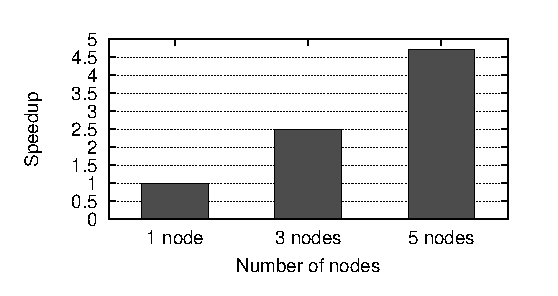
\includegraphics[width=0.35\textwidth]{grafici/graficoSpeedup.eps}
\caption{Speedup on the BigNetData dataset.}
\label{fig:speedup}
\end{figure}


\section{Conclusions and future perspectives}
\label{conclusion}
This paper presents a cloud-based service for discovering Misleading Generalized Itemsets from Big Data equipped with taxonomies.
To cope with Big Data the architecture has been designed to run on a distributed Hadoop architecture~\cite{Dean2008}.
A preliminary analysis of the applicability and usefulness of the proposed architecture was conducted on real Big Data 
acquired in a smart city environment and related to traffic law infractions.
However, the offered service could find application in many other application contexts, such as (i) social network analysis, 
(ii) network data analysis, and (iii) financial data analysis. 
As future work, we aim at optimizing and extending the current Hadoop architecture as well as testing its applicability in other real-life contexts. 



\bibliographystyle{IEEEtran}
\bibliography{biblio}

\end{document}